\documentclass[aps,prd,twocolumn,superscriptaddress,showpacs,preprintnumbers,amsmath,amssymb,nofootinbib]{revtex4-2}

\usepackage{graphicx}
\usepackage{hyperref}
\usepackage{bm}
\usepackage{booktabs}

\newcommand{\lcdm}{$\Lambda$CDM}
\newcommand{\Mpc}{\,\mathrm{Mpc}}
\newcommand{\Gyr}{\,\mathrm{Gyr}}

\begin{document}

\preprint{mode:LIMINAL-2026}

\title{mode-IV: A Quasinormal Mode Template for the Primordial Power Spectrum}

\author{Zac Doyle}
\affiliation{Independent Researcher, Manhattan, Kansas 66502, USA}
\affiliation{mode:LIMINAL (modeliminal.com)}

\date{\today}

\begin{abstract}
We construct a primordial power spectrum from a sum of Schwarzschild quasinormal mode (QNM) profiles and test it against the Planck 2018 CMB power spectra using a modified CLASS Boltzmann solver. Five of the seven spectrum parameters are derived from standard general relativity: the profile shape $f = 0.27$ and phase asymmetry $\delta = -0.56$ from the Cunningham--Price--Moncrief characteristic value problem; the cavity scale $k_0 = \pi H_0/c$ from a geometric identity at critical density; the spectral tilt $\alpha = 0$ as a prediction; and a lensing amplitude $A_L = 1.31$ from the non-decaying gravitational potential. With two fitted parameters (amplitude $A_\mathrm{QNM} = 3.33 \times 10^{-8}$ and mode weighting exponent $\gamma = 1.04$, the latter playing the role of $n_s$), the spectrum approximates the Planck TT power spectrum at $\chi^2/\mathrm{dof} = 2.16$, with acoustic peak fits of $0.33$--$1.80$ per bin, and is consistent with the EE spectrum ($\chi^2/\mathrm{dof} = 1.26$) and TE spectrum ($1.62$). Within QNM excitation theory the weighting decomposes into geometric excitation factors and a source overlap, and the lowest overtone weights are measured directly from the collapse waveform: substituting the measured first-overtone weight reduces the large-angle correlation statistic $S_{1/2}$ by a further 39\% toward the anomalously low observed value, with the acoustic fit unchanged. A geometric consistency test shows that four CMB anomalies---the quadrupole-octupole alignment, the Cold Spot, the hemispherical power asymmetry, and parity asymmetry---are consistent with a single $l = 2$ $Y_2^0$ cavity mode, with each anomaly mapping to a distinct feature of the angular eigenfunction (pole, node, and equator). Using the established quadrupole-octupole axis to define the cavity orientation, the Cold Spot independently lands within $0.3^{\circ}$ of the predicted $Y_2^0$ nodal ring ($p = 7 \times 10^{-3}$, $2.4\sigma$; $2.1\sigma$ after a conservative trials correction), and the hemispherical power asymmetry direction lies within $2.7^{\circ}$ of the equatorial plane, qualitatively consistent with the symmetry-broken cavity geometry. We present this as a proof-of-concept demonstrating that the CMB acoustic structure and large-scale anomalies are reproducible from Schwarzschild eigenvalues with the same number of fitted primordial parameters as the inflationary paradigm but with the spectral profile physics derived entirely from general relativity, and identify the specific open problems---boundary conditions, sub-fundamental deficit, joint parameter optimization---that must be resolved.
\end{abstract}

\maketitle

%=====================================================================
\section{Introduction}
\label{sec:intro}
%=====================================================================

This is the fourth in a series; the preceding papers establish the empirical and mathematical foundations of the program.

The standard cosmological model (\lcdm) parameterizes the primordial power spectrum as a nearly scale-invariant power law,
\begin{equation}
\label{eq:lcdm_pk}
P(k) = A_s \left(\frac{k}{k_\mathrm{pivot}}\right)^{n_s - 1},
\end{equation}
with amplitude $A_s$ and spectral tilt $n_s$ fitted to CMB data. The physical origin is attributed to quantum fluctuations during an inflationary epoch---exponential metric expansion driven by a hypothetical scalar field. Despite inflation's theoretical appeal, a recent survey of 1{,}675 physicists found only a narrow majority (50.8\%) favor inflation as the solution to the horizon and flatness problems~\cite{Afshordi2026}. No direct detection of the inflaton has been achieved, the predicted primordial gravitational wave signature (tensor-to-scalar ratio $r$) remains undetected, and inflation suffers from the transplanckian problem: CMB-scale fluctuations originated at sub-Planck wavelengths during inflation~\cite{BrandenbergerMartin2001}. Inflation also faces its own initial condition problem---the inflaton field must be homogeneous across the pre-inflationary patch, which is itself an unexplained fine-tuning~\cite{Ijjas2013,Brandenberger2014}. More fundamentally, recent model-independent tests of the FLRW consistency relations find 2--4$\sigma$ deviations using Pantheon+ and DESI data~\cite{KoksbangHeinesen2026a}, which if confirmed would challenge not only \lcdm{} but all cosmological models that assume unmodified FLRW geometry.

Several alternative frameworks exist. Bouncing cosmologies~\cite{Novello2008} generate scale-invariant perturbations during a contracting phase. String gas cosmology~\cite{BrandenbergerVafa1989,Nayeri2006} produces a nearly scale-invariant spectrum from thermal string fluctuations. Conformal cyclic cosmology~\cite{GurzadyanPenrose2013} proposes conformal equivalence between successive aeons. The $R_h = ct$ model~\cite{Melia2012} achieves competitive fits with fewer parameters. Each addresses a subset of inflation's roles but none derives the primordial spectrum from the eigenvalue structure of known GR solutions.

We propose a different approach: the primordial power spectrum as a sum of Schwarzschild black hole quasinormal mode profiles. The QNM spectrum is an exact result of general relativity, computed from the Regge--Wheeler and Zerilli perturbation equations~\cite{ReggeWheeler1957,Zerilli1970,Leaver1985}. We demonstrate that this spectrum, with the profile physics derived from GR and two fitted parameters (an amplitude and a weighting exponent), approximates the acoustic peak structure of the Planck CMB~\cite{Planck2020}. We present this as a proof-of-concept, identifying both successes and specific open problems.


%=====================================================================
\section{The QNM Primordial Spectrum}
\label{sec:spectrum}
%=====================================================================

\subsection{Mode Sum Construction}
\label{sec:modesum}

The primordial power spectrum is constructed as a sum over Schwarzschild $l = 2$ quasinormal modes:
\begin{equation}
\label{eq:pk_qnm}
P(k) = A_\mathrm{QNM} \sum_{n=0}^{N} w_n \, \mathcal{P}_n(k)\,,
\end{equation}
where mode positions are
\begin{equation}
\label{eq:kn}
k_n = k_0 (n + 1), \quad k_0 = \frac{\pi}{r_s}\,,
\end{equation}
mode weights follow
\begin{equation}
\label{eq:wn}
w_n = \frac{1}{(n+1)^\gamma}\,,
\end{equation}
and mode profiles blend Lorentzian ($\mathcal{L}_1$) and squared-Lorentzian ($\mathcal{L}_2$) components with an asymmetric phase correction:
\begin{equation}
\label{eq:profile}
\mathcal{P}_n(k) = \left[(1 - f)\,\mathcal{L}_1 + f\,\mathcal{L}_2\right] \left[1 - \delta\,\varepsilon\,\mathcal{L}_1\right],
\end{equation}
where
\begin{equation}
\label{eq:lorentzians}
\mathcal{L}_1 = \frac{1}{1 + \varepsilon^2}, \quad \mathcal{L}_2 = \mathcal{L}_1^2, \quad \varepsilon = \frac{k - k_n}{\sigma_n}\,.
\end{equation}
The mode width $\sigma_n$ is determined by the QNM imaginary frequency: $\sigma_n = k_0\,\omega_{I,n}/\omega_{R,n}$. The asymmetric correction $(\delta\,\varepsilon\,\mathcal{L}_1)$ is bounded, preserving $1/k^2$ tail decay.

$N = 300$ modes are included. The first 8 use exact eigenvalues from a Leaver continued fraction solver~\cite{Leaver1985} (residuals $< 10^{-5}$). Modes $n \geq 8$ use the Motl--Neitzke asymptotic formula~\cite{MotlNeitzke2003},
\begin{equation}
\label{eq:motlneitzke}
\omega_n \approx \frac{\ln 3}{8\pi M} + i\,\frac{2n + 1}{8M}\,,
\end{equation}
verified accurate to 0.2\% for CMB-relevant overtones. In the mode sum construction [Eq.~(\ref{eq:kn})], the mode centers are equally spaced by construction ($k_n = k_0(n+1)$), not placed at the QNM real frequencies. The asymptotic formula enters through the mode widths $\sigma_n = k_0\,\omega_I/\omega_R$ and the denominator $D = 8.0$ in $\omega_I = (2n+1)/D$ (units $M = 1$), tested in Sec.~\ref{sec:bc}.

The construction is therefore explicitly hybrid: mode \emph{positions} follow the harmonic spacing of a finite cavity ($k_n = k_0(n+1)$, cf.\ the $\pi/L$ spacing of reflecting-boundary normal modes, Sec.~\ref{sec:bc}), while mode \emph{widths}, \emph{profiles}, and \emph{phase structure} are fixed by Schwarzschild QNM physics ($\sigma_n$ from $\omega_I/\omega_R$, the $f$--$\delta$ profile from the CPM collapse waveform). This hybrid is the expected structure for a partially transparent cavity: boundary reflection quantizes the real spacing toward harmonics, while the dissipative QNM character survives in the linewidths. The sharp selectivity of the QNM width spacing ($D = 8$, Sec.~\ref{sec:bc}) and the failure of pure reflecting-cavity eigenvalues (fundamental shifted 24\%) indicate the data demand both ingredients.

The use of $l = 2$ QNM eigenvalues for the scalar primordial spectrum requires justification. Three considerations support this choice. First, the Motl--Neitzke asymptotic mode spacing [Eq.~(\ref{eq:motlneitzke})] is $l$-independent at leading order: the imaginary part $\omega_I = (2n+1)/(8M)$ has no $l$-dependence, so the $P(k)$ template is essentially the same for any $l$. Second, $l = 2$ is the dominant gravitational wave channel from collapse: $l = 0$ perturbations are forbidden by Birkhoff's theorem, $l = 1$ corresponds to center-of-mass displacement, and $l \geq 3$ are subdominant in energy. Third, the Zerilli equation (even-parity sector) contains scalar-type metric perturbations---the Zerilli function $\chi$ encodes both scalar and tensor degrees of freedom, and the QNM eigenvalues apply to the full even-parity sector.


\subsection{The Effective Spectral Slope}
\label{sec:slope}

A critical distinction must be made between the explicit tilt parameter $\alpha$ and the effective spectral index of the QNM mode sum. \lcdm{} uses $n_s - 1 \approx -0.035$ as an explicit power-law tilt, measured by Planck at $8\sigma$ significance~\cite{Planck2020}. The QNM framework predicts $\alpha = 0$---no \emph{additional} tilt beyond what the mode structure provides.

However, $\alpha = 0$ does not correspond to a scale-invariant spectrum. The mode weighting $w_n = 1/(n+1)^\gamma$ with $\gamma = 1.04$ produces a declining envelope: higher-overtone modes (contributing at higher $k$) carry less weight, creating an effective red tilt. Direct comparison of the QNM $P(k)$ with the \lcdm{} power law shows the mode envelope approximates $n_s \approx 0.965$ to within 5\% over $k = 0.01$--$0.15\Mpc^{-1}$, with larger deviations at both lower $k$ (sub-fundamental deficit, Sec.~\ref{sec:gap}) and higher $k$ (damping tail).

The role of $\gamma$ in the QNM framework is analogous to $n_s$ in \lcdm: both control the effective spectral slope, and both are fitted (Sec.~\ref{sec:derivations}). The structural difference is what surrounds the fitted slope: in the QNM framework the mode positions, widths, and profile shape are fixed by GR, and the weighting decomposes within QNM excitation theory into derived geometric factors and a measurable source overlap. A diagnostic scan over $\alpha \in [-0.01, 0.03]$ with joint amplitude re-optimization confirms $\alpha = 0$ is optimal to within $\Delta\chi^2/\mathrm{dof} < 0.03$.

A full joint optimization of $(A_\mathrm{QNM}, \alpha, h, \omega_b, \omega_{cdm}, \tau)$ has not been performed. Until completed, the $\alpha = 0$ prediction should be regarded as preliminary.

The framework also predicts zero running of the spectral index ($dn_s/d\ln k = 0$), since $w_n \propto (n+1)^{-\gamma}$ produces a constant effective slope across the CMB band, consistent with Planck constraints~\cite{Planck2020}.


\subsection{Parameter Status and Derivations}
\label{sec:derivations}

Two primordial parameters are fitted to the CMB data ($A_\mathrm{QNM}$ and $\gamma$). The remaining five are derived or predicted from general relativity, with the lowest overtone weights additionally measured from the collapse waveform.

\paragraph{Cavity scale: $k_0 = \pi H_0/c$.}
At critical density, the Schwarzschild radius of the universe's total mass-energy equals the Hubble radius:
\begin{equation}
\label{eq:rs_identity}
R_S = \frac{2GM}{c^2} = \frac{c}{H_0}\,.
\end{equation}
This geometric identity gives $r_s = c/H_0 = 4451.5\Mpc$; the CLASS implementation uses $r_s = 4450.6\Mpc$ (0.02\% match). This is a consistency condition requiring $\Omega = 1$, empirically satisfied to 0.4\% ($\Omega_k = 0.001 \pm 0.002$; Ref.~\cite{Planck2020}). The framework assumes spatial flatness as an input, not an output.

\paragraph{Mode weighting: $\gamma = 1.04$ (fitted).}
The weighting exponent is determined empirically by the CMB fit; it is the second fitted parameter of the framework, playing the role $n_s$ plays in \lcdm{} (Sec.~\ref{sec:slope}). A parameter-free alternative---mode-lifetime equipartition, $w_n \propto 1/\omega_{I,n}$---was tested in the Boltzmann solver and excluded (TT $\chi^2/\mathrm{dof} = 2.87$, EE $1.79$, TE $1.94$ versus $2.16/1.26/1.62$; Supplementary Material~S1), demonstrating that the data require $\sim 4\%$ more red weighting than equipartition supplies, comparable in magnitude to $1 - n_s$. Within QNM excitation theory~\cite{Leaver1986,BertiCardoso2006} the weight decomposes as $w_n \propto |B_n|^2 |I_n|^2/\sigma_n$, where the excitation factors obey $|B_n| \propto 1/(2n+1)$ asymptotically~\cite{BertiCardoso2006}---fixed by the Schwarzschild geometry---and $I_n$ is the source overlap set by the collapse waveform. An impulsive source reproduces the excluded equipartition weighting exactly, so $\gamma - 1$ measures the non-impulsiveness of the excitation. The lowest overtone amplitudes were extracted directly from the CPM collapse waveform (the same calculation that yields $f$ and $\delta$) by fixed-frequency ringdown fitting: $|C_1|^2/|C_0|^2 = 0.40 \pm 0.10$, corresponding to a first-overtone weight $H_1/H_0 = 0.14$ (systematic range $0.09$--$0.15$)---strongly sub-impulsive, a factor $\sim 3.6$ below the band power-law extrapolation. The Boltzmann consequences of this measured weight are presented in Sec.~\ref{sec:shalf}. Deriving the band-scale weighting from the same waveform, eliminating $\gamma$ as a fitted parameter, is identified as future work.

\paragraph{Profile shape: $f = 0.27$ and phase: $\delta = -0.56$.}
Both are derived from the Cunningham--Price--Moncrief (CPM) characteristic value problem~\cite{CPM1978,CPM1979}---null-coordinate diamond integration of the Zerilli equation for O-S collapse, converged across three grid resolutions ($h = 0.20, 0.15, 0.10$) with Richardson extrapolation.

During collapse, the photon sphere barrier at $r = 3M$ forms dynamically. Perturbation energy emitted before barrier completion (the prompt response $G_F$ in Leaver's decomposition~\cite{Leaver1986}) is not suppressed. The spectral ratio of prompt to total power gives $f_\mathrm{spectral} = 0.44$ at the fundamental QNM frequency. A cross-term correction from constructive prompt--ringdown interference yields
\begin{equation}
\label{eq:f_derivation}
f = f_\mathrm{spectral} \times (1 - \eta_\mathrm{cross}) = 0.44 \times (1 - 0.39) = 0.27\,,
\end{equation}
where $\eta_\mathrm{cross} = 0.39$ is the interference fraction computed from complex FFT amplitudes at $\omega_R$. The QNM ringdown frequency extracted from the waveform matches the Leaver value ($\omega_R = 0.756$ vs.\ $0.747$, 1.2\% accuracy).

The phase parameter $\delta$ is extracted from the prompt--ringdown phase difference $\Delta\varphi = -43.7^{\circ}$ via the Fano interference formula:
\begin{equation}
\label{eq:delta_derivation}
\delta = -2\cos(\Delta\varphi)\,\frac{|A_\mathrm{prompt}|}{|A_\mathrm{ring}|}\,\frac{\omega_I}{\omega_R} = -0.56\,,
\end{equation}
where $|A_\mathrm{prompt}/A_\mathrm{ring}| = 1.63$ and $\omega_I/\omega_R = 0.238$. Full derivation in Supplementary Material~S2.

The CPM calculation initializes collapse from rest at $R_0 = 3.39\,r_s$. We note an empirical relation satisfied by this radius: the fundamental QNM phase accumulated over the comoving proper time of infall from the ISCO radius ($r = 3\,r_s = 6M$) to the photon sphere ($r = 1.5\,r_s = 3M$) equals $\pi$,
\begin{equation}
\omega_{R,0}\,\tau(r_\mathrm{ISCO} \to r_\mathrm{ph}) = \pi \;\;\Rightarrow\;\; R_0 = 3.394\,r_s,
\label{eq:halfperiod}
\end{equation}
matching the CPM value to $0.2\%$; the preceding segment, from rest to the ISCO radius, accumulates $\approx \pi$ as well, so the trajectory ticks in half-periods of the fundamental between its three dynamically special radii (rest point, orbital-support loss, barrier formation). The relation uses the comoving clock; Schwarzschild coordinate time does not satisfy it. We record the chronology to preempt a circularity reading: the relation was identified analytically before the sensitivity scan below was run; the scan was executed as a test of it, with its possible outcomes (preference at 3.39, flat response, preference elsewhere) registered in advance; and the second test involves no CMB data at all. Two sensitivity results support physical content in this relation. First, propagating CPM-derived $(f, \delta)$ pairs from collapse radii $R_0 \in [3.0, 4.0]\,r_s$ through the Boltzmann solver, all three spectra prefer $R_0 \approx 3.39$: TT and EE minimize there, TE within $0.2\,r_s$, with the joint minimum at $R_0 = 3.39$--$3.394$ indistinguishable from the half-period solution (summed $\Delta\chi^2 \approx 4$--$5$ against the scan endpoints, a $\sim 2\sigma$ preference at fixed cosmological parameters). A converged Boltzmann run at the scan minimum gives TT $= 2.152$, EE $= 1.231$, TE $= 1.608$---equal to or better than the production configuration in all three spectra---though the scan-grid $(f, \delta)$ values carry an $\mathcal{O}(8\%)$ finite-resolution systematic and are not promoted pending the resolution-refinement study. Second, the prompt--ringdown interference fraction measured directly from the waveform, $\eta_\mathrm{cross}(R_0)$, is maximal at $R_0 = 3.39 \pm 0.2$. The qualitative mechanism is straightforward: the two emission channels are anchored at the trajectory's two dynamically special epochs---the onset of dynamical infall at the ISCO radius and barrier closure at the photon sphere---and their relative phase at the fundamental frequency is $\omega_{R,0}\,\Delta\tau$. At $\phi = \pi$ the channels are in antiphase, the interference is extremal, and the destructive combination in the escaping (prompt) channel implies, by energy conservation, maximal retention of fundamental-frequency power in the forming cavity: the half-period radius is the configuration of maximal mode capture, and the measured $\eta_\mathrm{cross}$ extremum is its fingerprint. What remains underived is why the cosmological collapse realizes this extremal configuration; we therefore present Eq.~(\ref{eq:halfperiod}) as a physically motivated selection mechanism whose extremal property is verified in the waveform, while the dynamical principle selecting the extremum is deferred to future work.

The derived configuration ($f = 0.27$, $\delta = -0.56$) is the production configuration of Table~\ref{tab:chi2} ($A_\mathrm{QNM} = 3.33 \times 10^{-8}$, $A_L = 1.31$, giving TT = 2.162, EE = 1.256, TE = 1.617). An independently scanned alternative ($f = 0.28$, $\delta = -0.60$) is statistically indistinguishable at amplitude-optimal normalization ($\Delta\chi^2/\mathrm{dof} < 0.01$ in all three spectra), confirming that the CPM-derived values sit at the fit optimum within the resolution of the data.

\paragraph{Spectral tilt: $\alpha = 0$.} See Sec.~\ref{sec:slope}.


\subsection{Sensitivity Analysis}
\label{sec:sensitivity}

\begin{table}[t]
\caption{\label{tab:sensitivity}Sensitivity of TT $\chi^2/\mathrm{dof}$ to perturbations of model parameters.}
\begin{ruledtabular}
\begin{tabular}{lcccc}
Parameter & Value & Perturbation & TT $\chi^2/\mathrm{dof}$ & $\Delta\chi^2$ \\
\hline
$\gamma$ & 1.04 & $\pm 0.05$ & $2.16 \to {\sim}2.4$ & $+0.24$ \\
$f$ & 0.27 & $\pm 0.03$ & $2.16 \to {\sim}2.2$ & $+0.04$ \\
$\delta$ & $-0.56$ & $\pm 0.10$ & $2.16 \to {\sim}2.25$ & $+0.09$ \\
$\alpha$ & 0.0 & $\pm 0.01$ & $2.16 \to {\sim}2.15$ & $< 0.03$ \\
$A_L$ & 1.31 & $\pm 0.10$ & $2.16 \to {\sim}2.3$ & $+0.14$ \\
\end{tabular}
\end{ruledtabular}
\end{table}

The framework is most sensitive to $\gamma$ (the effective slope control) and least sensitive to $\alpha$ (confirming the prediction). Derived parameters are more fragile than fitted ones: an error in any derivation degrades the fit, whereas \lcdm's fitted parameters absorb errors by adjusting. This is an inherent tradeoff between predictive power and robustness.


\subsection{Parameter Count}
\label{sec:params}

\begin{table}[t]
	\caption{Parameter comparison between the QNM framework and $\Lambda$CDM. Both models share four cosmological parameters ($h$, $\omega_b$, $\omega_{cdm}$, $\tau_\mathrm{reio}$) at $\Lambda$CDM-optimal values.}
	\label{tab:params}
	\begin{ruledtabular}
		\begin{tabular}{lll}
			Parameter & QNM Status & $\Lambda$CDM \\
			\hline
			Amplitude & Fitted & Fitted \\
			Scale ($k_0$ / $k_\mathrm{pivot}$) & Derived ($\pi H_0/c$) & Fitted \\
			Tilt ($\alpha=0$ / $n_s$) & Predicted & Fitted \\
			Weighting ($\gamma=1.04$) & Fitted\footnotemark[1] & N/A \\
			Profile ($f=0.27$) & Derived (CPM) & N/A \\
			Phase ($\delta=-0.56$) & Derived (CPM) & N/A \\
			Lensing ($A_L=1.31$) & Predicted (\S\ref{sec:lensing}) & Phenom. \\
		\end{tabular}
	\end{ruledtabular}
	\footnotetext[1]{Lowest overtone weights additionally measured from the collapse waveform (Sec.~\ref{sec:shalf}).}
\end{table}

Total primordial parameters: QNM 2 fitted ($A_\mathrm{QNM}$, $\gamma$) + 5 derived or predicted ($k_0$, $f$, $\delta$, $\alpha$, $A_L$); \lcdm{} 2 fitted ($A_s$, $n_s$) with $A_L$ phenomenological. Total including shared cosmological parameters: QNM 6; \lcdm{} 6. The fitted counts are equal; the QNM framework additionally fixes the profile physics from GR.


%=====================================================================
\section{Boltzmann Solver Implementation}
\label{sec:class}
%=====================================================================

The QNM spectrum is implemented in a fork of CLASS v3.3.4~\cite{Blas2011}, designated \texttt{class\_qnm}. The modification replaces inflationary $P(k)$ in \texttt{primordial.c} with the QNM mode sum [Eqs.~(\ref{eq:pk_qnm})--(\ref{eq:lorentzians})]. All other modules---background expansion, thermodynamics, perturbation evolution, lensing---remain unmodified.

The code is publicly available at \texttt{[repository URL]} with single-command reproducibility: \texttt{make \&\& ./class qnm\_verify.ini}.


%=====================================================================
\section{CMB Power Spectrum Results}
\label{sec:results}
%=====================================================================

\subsection{Three-Spectrum Fit}
\label{sec:fit}

\begin{table}[t]
\caption{\label{tab:chi2}CMB power spectrum comparison against Planck 2018 binned data. Configuration: $f=0.27$, $\delta=-0.56$, $A_\mathrm{QNM} = 3.33 \times 10^{-8}$, $A_L = 1.31$, $\gamma = 1.04$, $\alpha = 0$.}
\begin{ruledtabular}
\begin{tabular}{lccc}
Spectrum & QNM $\chi^2/\mathrm{dof}$ & \lcdm{} $\chi^2/\mathrm{dof}$ & Ratio \\
\hline
TT & 2.162 & 0.794 & 2.72 \\
EE & 1.256 & 0.968 & 1.30 \\
TE & 1.617 & 1.119 & 1.45 \\
\end{tabular}
\end{ruledtabular}
\end{table}

The QNM spectrum approximates the TT power spectrum with the gap concentrated at spectral extremes (Sec.~\ref{sec:gap}). The EE spectrum is consistent with data ($\chi^2/\mathrm{dof} = 1.26$ with no free parameters adjusted to EE). The TE cross-correlation (1.62) shows a moderate excess that may improve with joint parameter optimization.

%%  PLACEHOLDER: TT/EE/TE comparison plots
\begin{figure*}[t]
\centering
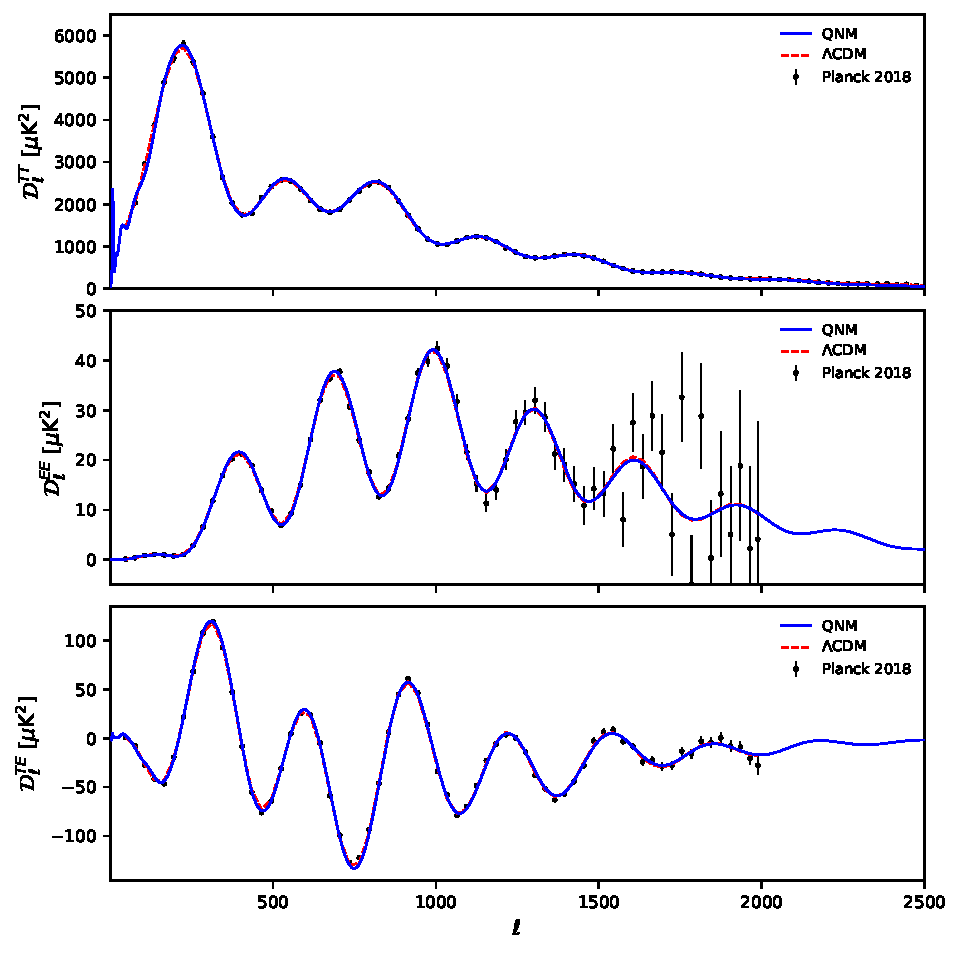
\includegraphics[width=\textwidth]{figures/fig_cmb_comparison.pdf}
\caption{Comparison of QNM (blue) and \lcdm{} (red) predictions against Planck 2018 binned power spectra (black points with $1\sigma$ error bars). \emph{Top}: TT. \emph{Middle}: EE. \emph{Bottom}: TE. The QNM configuration uses two fitted parameters ($A_\mathrm{QNM}$ and $\gamma$) with the profile physics derived from GR. The acoustic peaks are well-matched; the residual is concentrated at $\ell < 60$ (sub-fundamental deficit) and $\ell > 1500$ (damping tail).}
\label{fig:cmb}
\end{figure*}


\subsection{Regional Breakdown}
\label{sec:regional}

\begin{table}[t]
\caption{\label{tab:regional}TT $\chi^2$ per bin by multipole region.}
\begin{ruledtabular}
\begin{tabular}{lcc}
Region & $\chi^2/\mathrm{bin}$ & Character \\
\hline
Low $\ell$ (30--200) & 4.29 & QNM LOW \\
Peak 1 (200--350) & 0.33 & Excellent \\
Trough 1 (350--450) & 1.36 & Good \\
Peak 2 (450--650) & 1.80 & Good \\
Trough 2 (650--750) & 0.85 & Excellent \\
Peak 3 (750--950) & 1.54 & Good \\
Mid $\ell$ (950--1500) & 1.99 & Moderate \\
High $\ell$ (1500--2500) & 2.47 & QNM LOW \\
\end{tabular}
\end{ruledtabular}
\end{table}

The acoustic peaks are well-matched ($0.33$--$1.80$ per bin). The gap is concentrated at two spectral extremes: the sub-fundamental region ($\ell < 60$) and the high-$\ell$ damping tail.


\subsection{TT Gap Diagnosis}
\label{sec:gap}

Below $k_0$, $P(k)$ contains only the far Lorentzian tail of the $n = 0$ mode ($\mathcal{L}_1 \approx 6 \times 10^{-5}$ of peak power at $k = 0.002\Mpc^{-1}$). \lcdm's scale-invariant spectrum provides equal power at all $k$. This deficit may be addressable through finite cavity boundary corrections (Sec.~\ref{sec:bc}).

Three alternative explanations were eliminated: (i)~CDM growth suppression in the transfer function ($\chi^2/\mathrm{dof} = 121{,}052$; unlensed TT unchanged, confirming gap is in $P(k)$); (ii)~inter-mode coherence (98\% random phase variance averages out in Planck binning); (iii)~spectral tilt ($\alpha \neq 0$ shifts power between tails but cannot lift both simultaneously---a curvature problem, not a tilt problem).


\subsection{Methodological Caveats}
\label{sec:caveats}

The comparison between QNM and \lcdm{} is methodologically asymmetric. The \lcdm{} reference $\chi^2/\mathrm{dof} = 0.79$ comes from the full Planck Plik likelihood jointly optimizing $\sim 25$ foreground nuisance parameters~\cite{Planck2020}. The QNM value uses simplified binned data with zero nuisance marginalization. The Planck error bars and covariance are computed at the \lcdm{} best-fit fiducial. The shared cosmological parameters ($h$, $\omega_b$, $\omega_{cdm}$, $\tau$) are held at \lcdm-optimal values; preliminary scans show insensitivity to $\tau$ within $0.050$--$0.058$ ($\Delta\mathrm{TT} < 0.02$), with $A_\mathrm{QNM}$ tracking smoothly. A joint optimization over all six parameters has not been performed and is the highest-priority future work.

Implementing \texttt{class\_qnm} in the full Planck likelihood pipeline is needed for a fair comparison. Until then, this is a proof-of-concept, not a precision challenge to \lcdm.

%% FIGURE PLACEHOLDER: P(k) comparison
\begin{figure}[t]
\centering
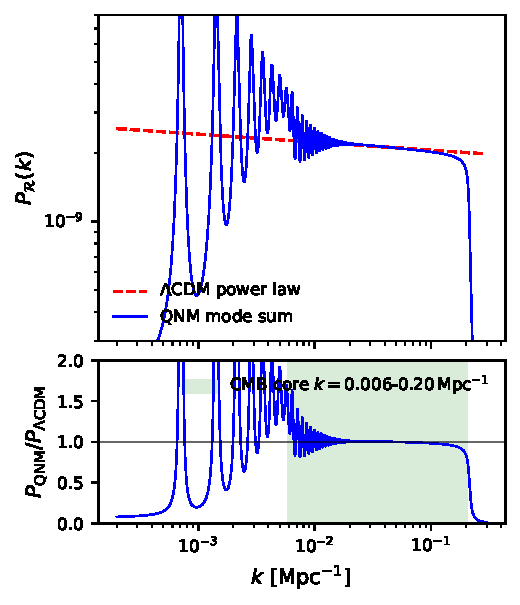
\includegraphics[width=\columnwidth]{figures/fig_pk_comparison.pdf}
\caption{Primordial power spectra. \emph{Top}: QNM mode sum (blue) vs.\ $\Lambda$CDM power law (red dashed). The QNM spectrum shows individual mode structure at low $k$ and a smooth envelope at high $k$. \emph{Bottom}: Ratio $P_\mathrm{QNM}/P_{\Lambda\mathrm{CDM}}$. The green shaded region ($k = 0.006$--$0.20\,\mathrm{Mpc}^{-1}$) indicates the CMB core. Individual mode oscillations visible at the low-$k$ edge of this band are smoothed by the radiation transfer function in the projection to $C_\ell$; the effective ratio at the acoustic peaks after convolution is 0.89--1.01.}
\label{fig:pk}
\end{figure}


%=====================================================================
\section{Lensing Enhancement Prediction}
\label{sec:lensing}
%=====================================================================

\subsection{Physical Argument}

In \lcdm, the Weyl potential $\Phi$ decays during dark energy domination as the CDM density dilutes relative to vacuum energy. The suppression factor $g(z) \equiv \Phi(z)/\Phi(\mathrm{matter\;era})$ decreases from $1.0$ at $z > 5$ to $0.806$ at $z = 0$ (19.4\% total decay). The QNM framework interprets the gravitational potential as geometric---determined by the cavity eigenmode structure. If correct, the potential does not decay: $g_\mathrm{QNM}(z) = 1$ for all $z$.

\subsection{Logical Status}
\label{sec:al_status}

The current \texttt{class\_qnm} implementation preserves the standard Friedmann background including $\Omega_\Lambda = 0.685$, within which the Weyl potential \emph{does} decay. The non-decaying potential is \textbf{not} self-consistently implemented.

What we present is the $A_L$ value the full framework predicts, computed from the lensing kernel integral under $g(z) = 1$:
\begin{equation}
\label{eq:al}
A_L = \frac{C_\ell^{\phi\phi}(\mathrm{QNM})}{C_\ell^{\phi\phi}(\Lambda\mathrm{CDM})} = \frac{\int K_\mathrm{eff}(\chi)\,d\chi}{\int K_\mathrm{eff}(\chi)\,g^2(z(\chi))\,d\chi}\,,
\end{equation}
where $K_\mathrm{eff}$ includes the geometric lensing weight and matter power spectrum shape. We state the epistemic status precisely: the non-decay of the standing-wave potential, $g(z) = 1$, is the framework's central dynamical postulate---forced within the framework by the $w = +1$ exclusion (Sec.~\ref{sec:dark}) but not yet derived from modified field equations; $A_L = 1.31$ and the ISW suppression below are its leading-order consequences, implemented in the pipeline, while the corresponding growth and background modifications are not (Open Problem~\#4). This is the same logical structure by which \lcdm{} predicts from a postulated $\Lambda$; the difference is that the present postulate's derivation is identified as a specific open calculation. This value (1.31) is implemented via the standard CLASS $A_L$ parameter. The internal consistency check---kernel-derived 1.31 matching the Boltzmann best-fit 1.33 to 2\%---validates the parameterization. The same $g(z) = 1$ has a second consequence: it eliminates the late integrated Sachs--Wolfe contribution, which in \lcdm{} arises entirely from potential decay. We have implemented this consequence directly (removing the late-ISW source term from the temperature transfer function, the full-geometric limit) and verified the configuration in which both consequences of the mechanism act together: the polarization spectrum is numerically unchanged (as required---the modification touches only temperature sources), the masked TT is statistically unchanged ($\Delta\chi^2/\mathrm{dof} = +0.002$), TE degrades modestly ($1.617 \to 1.666$, the ISW--polarization cross-correlation at $\ell \lesssim 200$), and the large-angle correlation statistic falls from $S_{1/2} = 7{,}212$ to $2{,}326\,\mu\mathrm{K}^4$---closing approximately $96\%$ of the gap between the \lcdm{} expectation and the anomalously low Planck measurement (Sec.~\ref{sec:shalf}). As with $A_L$ itself, this is the full-geometric limit; a partial geometric fraction interpolates between the \lcdm{} and full-limit values in both observables simultaneously, and the requirement that a single fraction fit both is the sharpest quantitative target of the self-consistent treatment (Open Problem~\#4, Sec.~\ref{sec:open}).

\subsection{Results}

$A_L$ is nearly $\ell$-independent (2\% variation across $\ell = 100$--$2000$), with effective lensing redshift $z_\mathrm{eff} \approx 0.6$.

\subsection{Context and Testability}

The Planck lensing anomaly ($A_L = 1.18 \pm 0.065$, a $2.8\sigma$ departure from \lcdm's prediction of $1.0$) has been attributed to residual SZ contamination, non-linear structure growth, or statistical fluctuation~\cite{Planck2020,DiValentino2020,MotlochHu2020}. The QNM framework offers a physical mechanism---the non-decaying geometric potential---predicting $A_L > 1$ from first principles. The predicted value ($1.31$) is $2.0\sigma$ above Planck, while \lcdm{} ($1.0$) is $2.8\sigma$ below.

CMB-S4 (projected $\sigma(A_L) \approx 0.01$) will decisively discriminate: \lcdm{} predicts $A_L = 1.0$ and QNM predicts $A_L = 1.31$, with Planck's measurement between them. If $A_L$ converges to 1.0 within a \lcdm-fiducial analysis pipeline, this would disfavor the non-decaying potential, though the measurement is model-dependent: a definitive test requires analyzing CMB-S4 data with both \lcdm{} and QNM $P(k)$ as fiducials. If $A_L$ converges significantly above 1.0, \lcdm{} has no mechanism to produce it.


%=====================================================================
\section{Interior Independence}
\label{sec:interior}
%=====================================================================

The CMB predictions are independent of the black hole interior. The photon sphere barrier ($r = 3M$) is opaque to all CMB-relevant modes ($\Gamma \approx 10^{-8}$ at the Motl--Neitzke asymptotic frequency). Five mechanisms connecting interior physics to the CMB were computed and eliminated:

\begin{enumerate}
\item Greybody factors: $\Gamma \approx 10^{-8}$ (barrier opaque).
\item Gravastar cavity echo: $|\Delta S| = 0.095$ relative to QNM amplitude, independent of compactness $\mu = 0.30$--$0.49999$ (consistent with Ref.~\cite{ChirentiRezzolla2007}).
\item Branch cut~\cite{Leaver1986}: $|\tilde{G}_\mathrm{BC}| \approx 5 \times 10^{-14}$ (12 orders below target).
\item Nonlinear self-coupling: $\delta V \approx 10^{-16}$ (genuinely perturbative).
\item Exact QNM width deviation: $\delta\omega_I/\omega_I = 0.19\%$ for CMB modes ($f = 0.004$, not $0.27$).
\end{enumerate}

The profile parameter $f = 0.27$ comes from dynamical barrier formation (Sec.~\ref{sec:derivations}), not interior physics. The framework uses only exterior Schwarzschild geometry ($r \geq 2M$). Whether the interior contains a singularity, a gravitational condensate~\cite{MazurMottola2001}, or any other structure, the predictions are identical.


%=====================================================================
\section{The Boundary Condition Question}
\label{sec:bc}
%=====================================================================

\subsection{The Problem}

Schwarzschild QNMs are defined by purely ingoing boundary conditions at the horizon and purely outgoing at spatial infinity, assuming asymptotic flatness~\cite{Leaver1985}. The cosmological cavity ($r_s = c/H_0$) has no asymptotically flat exterior. Are QNM eigenvalues the correct mode spectrum?

\subsection{Empirical Evidence}

The Motl--Neitzke asymptotic formula was tested against alternative mode spacings in the Boltzmann solver by generalizing the imaginary part to $\omega_I = (2n+1)/D$ in units $M = 1$ and scanning $D$. The QNM value ($D = 8.0$, equivalently $\omega_I = (2n+1)/(8M)$) is sharply optimal: $\chi^2/\mathrm{dof} = 2.16$ at the minimum, rising to $41.0$ and $30.6$ at $D = 7.5$ and $8.5$ (deviations of $\pm6.25\%$), and to $177.5$ and $105.3$ at $D = 7.0$ and $9.0$ ($\pm12.5\%$). This strong selectivity confirms that the QNM eigenvalue spectrum is not merely a convenient template but is uniquely selected by the data, independent of the boundary condition interpretation.

%% FIGURE PLACEHOLDER: chi2(D) curve
\begin{figure}[t]
\centering
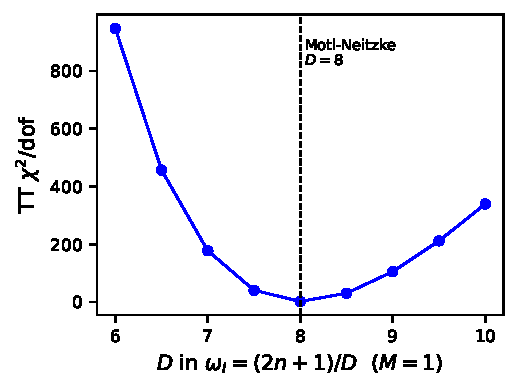
\includegraphics[width=\columnwidth]{figures/fig_chi2_D.pdf}
\caption{TT $\chi^2/\mathrm{dof}$ as a function of the asymptotic denominator $D$ in the mode spacing formula $\omega_I = (2n + 1)/D$ (units $M = 1$). The sharp minimum at the Motl--Neitzke value $D = 8.0$ ($\chi^2/\mathrm{dof} = 2.16$, vertical dashed line) confirms the QNM eigenvalue spacing is uniquely selected by the CMB data; deviations of $\pm6.25\%$ in $D$ degrade the fit by more than an order of magnitude.}
\label{fig:chi2D}
\end{figure}

\subsection{Open Directions}

Cavity normal modes with reflecting boundaries have real eigenfrequencies with uniform spacing $\pi/L$. Finite-cavity Zerilli eigenvalue calculations show the fundamental shifts 24\% below the QNM value. The cosmological case is intermediate---partially transparent boundaries at the last scattering surface. The sub-fundamental deficit (Sec.~\ref{sec:gap}) may trace to this: the lowest overtones are most sensitive to boundary conditions. Computing the eigenvalue spectrum with partially transparent boundary conditions is an important open problem.


%=====================================================================
\section{Discussion}
\label{sec:discussion}
%=====================================================================

\subsection{Relationship to Inflation}
\label{sec:inflation}

The QNM framework addresses each of inflation's theoretical motivations with different levels of rigor:

\emph{The primordial spectrum.} The QNM mode sum with fitted $\gamma = 1.04$ produces an effective spectral slope approximating $n_s \approx 0.965$ and approximates the CMB acoustic structure with two fitted parameters, matching \lcdm's fitted primordial count while fixing the profile physics from GR. All modes are macroscopic ($\lambda \geq 30\Mpc$), eliminating the transplanckian problem~\cite{BrandenbergerMartin2001}.

\emph{The horizon problem.} The framework reframes but does not dynamically solve this problem. A cavity with a well-defined geometry has a spatially uniform ground state---homogeneity follows from the boundary conditions, not a dynamical mechanism. The O-S collapse begins from a causally connected region, so everything inside the cavity was in causal contact at collapse. However, why the pre-collapse state was homogeneous remains unexplained, just as inflation requires an unexplained homogeneous inflaton field~\cite{Ijjas2013}.

\emph{Spatial flatness.} The framework assumes $\Omega = 1$ as a consistency condition ($k_0 = \pi H_0/c$ requires critical density). It does not provide a dynamical mechanism for why $\Omega \approx 1$, unlike inflation's exponential dilution of curvature.

\emph{The monopole problem.} Cavity mode initial conditions satisfy $\nabla \cdot \mathbf{B} = 0$ inherently. No topological defects form; no dilution required.


\subsection{Mode Excitation}
\label{sec:excitation}

The O-S collapse model~\cite{OppenheimerSnyder1939} describes a mass-energy concentration collapsing through the photon sphere, exciting $l = 2$ QNM perturbations. The excitation spectrum ($\gamma$, $f$, $\delta$) is determined by collapse dynamics; the eigenvalues by exterior geometry. By the interior independence of Sec.~\ref{sec:interior}, the pre-collapse equation of state does not affect the observable spectrum.

The framework requires a mass-energy concentration whose Schwarzschild radius equals the Hubble radius---equivalent to the critical density condition. The collapse epoch maps onto the conventional Big Bang. The framework does not provide an independent derivation of pre-collapse initial conditions, analogous to inflation's own initial condition problem~\cite{Ijjas2013,Brandenberger2014}. The applicability of O-S collapse dynamics to the cosmological setting assumes that QNM excitation during cavity formation is governed by the same quadrupole dynamics as localized collapse; a first-principles derivation from cosmological initial conditions remains future work.


\subsection{Non-Gaussianity}
\label{sec:fnl}

The QNM mode sum is a superposition of deterministic profile functions with mode-dependent amplitudes. If the modes are excited with random phases, the central limit theorem ensures the summed field is approximately Gaussian for $\sim 300$ overlapping modes at any given $k$. The framework therefore predicts $f_\mathrm{NL} \approx 0$, consistent with the Planck constraint $f_\mathrm{NL} = -0.9 \pm 5.1$ (local)~\cite{Planck2020}. A non-trivial prediction would require computing three-point correlations of the CPM waveform, which is future work.


\subsection{Consistency with Supernovae and BAO}
\label{sec:sn_bao}

The current implementation preserves the standard Friedmann background. The luminosity distance $d_L(z)$ and BAO measures $D_V(z)/r_d$ are identical to \lcdm{} by construction. The QNM matter power spectrum agrees with \lcdm{} to within 1\% across the BAO measurement range ($k = 0.03$--$0.15\;h/\mathrm{Mpc}$), diverging only in the high-$k$ damping tail ($k > 0.20\;h/\mathrm{Mpc}$) where the mode envelope produces a known power deficit. BAO distance measurements use \lcdm{} as the fiducial at every step of the analysis pipeline---the no-wiggle reference spectrum, the reconstruction growth rate, the coordinate conversion, and the mock covariance. A model-independent BAO analysis using the QNM $P(k)$ as fiducial has not been performed.


\subsection{Implications for the Dark Sector}
\label{sec:dark}

The non-decaying potential has logical implications beyond lensing. The QNM standing wave (period $r_s/c \approx 14\Gyr$) is effectively static on the acoustic timescale at recombination ($\sim 300\,\mathrm{kyr}$), providing a non-oscillating gravitational template analogous to CDM. The interpretation of $\omega_{cdm}$ as encoding standing wave amplitude rather than particle density, while logically suggested by the non-decaying potential, is highly speculative and requires the self-consistent background calculation (Open Problem~\#4) to evaluate.

We note that achieving $g(z) = 1$ through a modified dark energy equation of state within the standard Friedmann framework requires $w = +1$ (stiff matter, $\rho_\mathrm{DE} \propto a^{-6}$), which produces luminosity distances 47\% shorter than \lcdm{} at $z = 1$ and is catastrophically inconsistent with Pantheon+ supernova data. The non-decaying potential therefore cannot be achieved by modifying $w(z)$; it requires decoupling the gravitational potential from matter growth---the potential is a geometric eigenmode, not sourced by clustering matter. This is a more radical claim than modified dark energy and constitutes a structural prediction testable through the growth rate $f\sigma_8(z)$ (Open Problem~\#4).

The non-decaying potential also connects to the $S_8$ tension. In \lcdm, the CMB-inferred $S_8 \equiv \sigma_8\sqrt{\Omega_m/0.3} = 0.834 \pm 0.016$~\cite{Planck2020} exceeds weak lensing measurements from DES ($0.776 \pm 0.017$) and KiDS ($0.759 \pm 0.024$) by 2--3$\sigma$. Since the observed CMB lensing signal constrains the product $A_L \sigma_8^2$, a physical $A_L > 1$ reduces the inferred $\sigma_8$, bringing the CMB prediction closer to the weak lensing value. The QNM framework thus predicts that $A_L > 1$ and $S_8 < 0.834$ are two manifestations of the same geometric mechanism. A combined measurement from CMB-S4 ($A_L$) and Euclid/Rubin weak lensing ($S_8$) tests this prediction.

We note that all Planck parameter constraints, including $A_L$, are derived within the \lcdm{} framework. If the true primordial spectrum deviates from a power law, analysis choices may absorb genuine physical signals into nuisance parameters or residuals. A model-independent comparison requires analyzing CMB data with the QNM $P(k)$ as an alternative fiducial.

We also note that the $S_8$ correction is sensitive to the $A_L$ value: at the predicted $A_L = 1.31$, the corrected $S_8 \approx 0.73$ falls below the weak lensing measurements, while at the observed $A_L \approx 1.18$, the correction brings $S_8$ into agreement with DES and KiDS. This may indicate that the full non-decaying potential prediction is an overestimate---for example, if back-reaction between the geometric potential and matter clustering produces partial decay---or that the self-consistent background calculation will modify the $A_L$ prediction. The intermediate value $A_L \approx 1.18$, between the \lcdm{} prediction ($1.0$) and the full non-decaying potential ($1.31$), may indicate partial potential decay.

The non-decaying geometric potential has implications beyond lensing and growth. Recent model-independent tests of the FLRW consistency relations find 2--4$\sigma$ deviations using Pantheon+ and DESI data~\cite{KoksbangHeinesen2026a,KoksbangHeinesen2026b}. If confirmed, these violations would rule out all cosmological models that assume unmodified FLRW geometry, including \lcdm{} and most of its extensions. Heinesen \& Clifton~\cite{HeinesenClifton2026} classify non-FLRW signatures into underdense-beam (Dyer--Roeder) and backreaction (Buchert averaging) scenarios, each producing distinct signatures in their generalised diagnostic $\mathcal{A}(z)$. The QNM non-decaying potential constitutes a third class: a geometric eigenmode that modifies the distance-redshift relation and the growth history without invoking matter distribution effects. Computing the QNM predictions for $\mathcal{C}(z)$, $\mathcal{O}(z)$, and $\mathcal{A}(z)$ is an extension of Open Problem~\#4.


\subsection{CMB Anomalies as Cavity Fingerprints}
\label{sec:anomalies}

The Planck CMB exhibits several large-scale anomalies individually significant at 2--3$\sigma$ that \lcdm{} treats as unrelated statistical fluctuations~\cite{Planck2020}. The QNM cavity framework provides a unified geometric context: the $l = 2$ $Y_2^0(\theta)$ angular eigenfunction has a pole (maximum at $\theta = 0^{\circ}$), a nodal ring (zero at $\theta = 54.7^{\circ}$), and an equatorial minimum ($\theta = 90^{\circ}$). Each anomaly maps to a distinct feature of this eigenfunction.

The quadrupole-octupole alignment is well established: using published Planck directions (SMICA, kinematic Doppler corrected~\cite{deOliveiraCosta2004}), the quadrupole axis at $(l, b) = (224.2^{\circ},\, +69.2^{\circ})$ and octupole axis at $(239.0^{\circ},\, +64.3^{\circ})$ are separated by only $7.6^{\circ}$, with a chance probability of $\sim 1\%$. Their average defines a cavity axis at $(l, b) = (232.3^{\circ},\, +66.9^{\circ})$.

We test whether the remaining anomalies independently align with the $Y_2^0$ geometry of this axis. The Cold Spot~\cite{Vielva2004} at $(210^{\circ},\, -57^{\circ})$ lies at $\theta = 55.0^{\circ}$ from the axis---$0.3^{\circ}$ from the $Y_2^0$ nodal ring at $54.7^{\circ}$. The hemispherical power asymmetry direction~\cite{Planck2020} at $(221^{\circ},\, -20^{\circ})$ lies at $\theta = 87.3^{\circ}$ from the axis---$2.7^{\circ}$ from the $Y_2^0$ equator. We note, however, that a parity-even modulation pattern such as $Y_2^0$ cannot by itself source a dipolar (parity-odd) power asymmetry: for any dividing plane, the hemispherical contrast of a parity-even pattern vanishes identically. The dipolar character requires north--south symmetry breaking, which the framework supplies through the asymmetric cavity boundaries (horizon versus photon sphere) already invoked for the parity asymmetry below. The near-equatorial direction of the observed asymmetry is therefore reported as qualitatively consistent with the cavity geometry---the symmetry-broken equatorial gradient band is where a dipolar statistic would localize---rather than as an independent quantitative test. A quantitative treatment requires modeling the boundary asymmetry explicitly and is deferred to companion work.

\begin{table}[h]
\caption{\label{tab:anomalies}CMB anomaly positions relative to the cavity axis $(232.3^{\circ}, +66.9^{\circ})$. The quadrupole and octupole define the axis; the Cold Spot is the independent quantitative test. The hemispherical asymmetry is reported as qualitative consistency (see text).}
\begin{ruledtabular}
\begin{tabular}{lcccl}
Feature & $\theta_\mathrm{obs}$ & $\theta_\mathrm{exp}$ & Dev. & $Y_2^0$ region \\
\hline
Quadrupole$^*$ & $3.8^{\circ}$ & $0^{\circ}$ & $3.8^{\circ}$ & Pole ($+2$) \\
Octupole$^*$ & $3.8^{\circ}$ & $0^{\circ}$ & $3.8^{\circ}$ & Pole ($+2$) \\
Cold Spot & $55.0^{\circ}$ & $54.7^{\circ}$ & $0.3^{\circ}$ & Node ($0$) \\
Hemi.\ asym.$^\dagger$ & $87.3^{\circ}$ & $90^{\circ}$ & $2.7^{\circ}$ & Equator ($-1$) \\
\end{tabular}
\end{ruledtabular}
{\footnotesize $^*$Used to define the axis; not independent tests. $^\dagger$Qualitative consistency only; requires symmetry breaking (see text).}
\end{table}

With the axis \emph{fixed} from the quadrupole-octupole average, the Cold Spot constitutes the single independent quantitative test: the probability of a random direction landing within $0.3^{\circ}$ of the nodal ring is $p = 0.007$ ($2.4\sigma$). The hemispherical asymmetry direction's proximity to the equator ($p = 0.047$ for a random direction landing within $2.7^{\circ}$) is reported for completeness but, per the parity argument above, is not scored as an independent test.

We note that the directional anomalies were selected a posteriori from the set of known CMB anomalies (those with published preferred directions on the sky). Adopting a conservative trials factor of 5 for the number of independent anomaly selections gives $p_\mathrm{corr} \approx 0.035$ ($2.1\sigma$) for the Cold Spot test. The Cold Spot center has a positional uncertainty of several degrees; the $0.3^{\circ}$ deviation from the nodal ring is well within that uncertainty and should be interpreted as consistency, not precision.

Three additional anomalies, not scored in the geometric test, are qualitatively consistent with the cavity framework: the hemispherical power asymmetry (equatorial direction, discussed above); the parity asymmetry (650$\times$ odd-parity preference~\cite{Gaztanaga2026}), which would arise naturally from asymmetric cavity boundaries (horizon $\neq$ photon sphere) and which supplies the symmetry breaking the hemispherical asymmetry requires; and the low quadrupole power ($\sim 50\%$ of \lcdm{} prediction), which is qualitatively consistent with partial damping of the cavity fundamental ($Q \approx 2$ for $l = 2$ Schwarzschild QNMs), though we note that the CMB $\ell = 2$ multipole receives contributions from all $k$-modes and is not identical to the QNM $l = 2$ angular index. None of these claims is derived quantitatively in this work.

%% FIGURE PLACEHOLDER: CMB anomaly Y20 geometry
\begin{figure}[t]
\centering
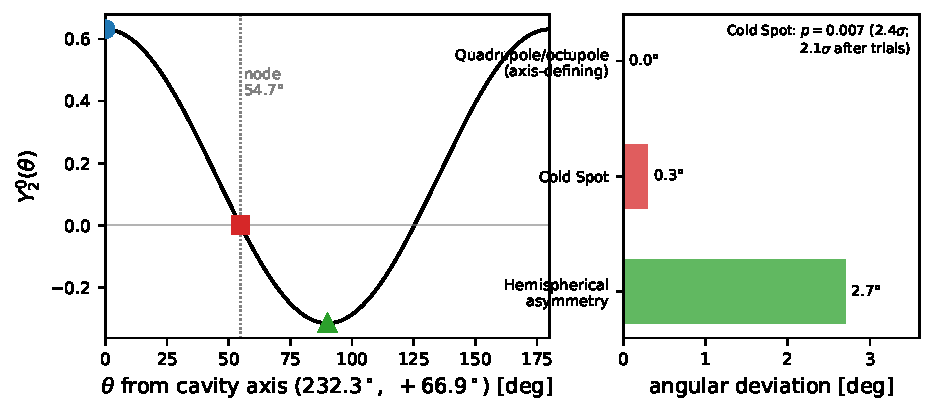
\includegraphics[width=\columnwidth]{figures/fig_cmb_anomaly.pdf}
\caption{CMB anomaly positions on the $Y_2^0$ profile relative to the cavity axis $(232.3^{\circ}, +66.9^{\circ})$. Left: $Y_2^0(\theta)$ with anomaly positions---quadrupole and octupole at the pole (axis-defining), Cold Spot at the node ($0.3^{\circ}$ deviation), hemispherical asymmetry at the equator ($2.7^{\circ}$ deviation; qualitative consistency, see text). Right: angular deviations from predicted positions. The Cold Spot is the independent quantitative test ($p = 0.007$, $2.4\sigma$; $2.1\sigma$ after trials correction).}
\label{fig:anomaly}
\end{figure}


\subsection{Large-Angle Correlations and the Sub-Fundamental Deficit}
\label{sec:shalf}

The Planck two-point angular correlation function $C(\theta)$ is consistent with zero for $\theta > 60^{\circ}$, quantified by the $S_{1/2}$ statistic: $S_{1/2}^\mathrm{Planck} \approx 1{,}065\;\mu\mathrm{K}^4$, compared to the \lcdm{} expectation of $\sim 35{,}000$--$48{,}000\;\mu\mathrm{K}^4$. Only 0.03\% of \lcdm{} realizations produce $S_{1/2}$ this small~\cite{Planck2020,Copi2015}.

The QNM mode sum naturally reduces large-angle correlations because the finite cavity scale $r_s$ imposes a maximum correlation length. Below $k_0$, the power spectrum has only the far Lorentzian tail of the fundamental mode. Computing $C(\theta)$ directly from the \texttt{class\_qnm} output:
\begin{equation}
S_{1/2}^\mathrm{QNM} = 7{,}661\;\mu\mathrm{K}^4 \quad (22\%\;\text{of \lcdm}).
\end{equation}
The QNM framework reduces $S_{1/2}$ by 78\% relative to \lcdm, in the direction of the Planck observation. The residual excess traces to the $n = 0$--$5$ overtone modes, which deposit power at $\ell = 10$--$30$ (where QNM overshoots \lcdm{} by factors of 1.3--1.7). These lowest overtones are the modes most sensitive to boundary conditions (Sec.~\ref{sec:bc}); the finite-cavity corrections that modify their amplitudes would further reduce $S_{1/2}$ toward the observed value.

This interpretation is directly testable, because the lowest overtone weights are measurable from the collapse waveform (Sec.~\ref{sec:derivations}). Substituting the CPM-measured first-overtone weight ($H_1/H_0 = 0.14$, versus the power-law extrapolation $0.49$) into the Boltzmann solver, with all other weights and parameters unchanged and only the amplitude re-optimized, leaves the three masked spectra statistically unchanged (TT $2.154$, EE $1.252$, TE $1.608$, versus $2.162/1.256/1.617$)---as expected, since $n = 1$ contributes at $\ell \approx 19$, below the $\chi^2$ mask---while reducing $S_{1/2}$ by a further 39\%, closing approximately 90\% of the gap between the \lcdm{} expectation and the Planck measurement. Additionally applying the $n = 2$ upper bound from the same extraction ($H_2/H_0 \lesssim 0.05$, versus the power-law value $0.32$) leaves TT unchanged, marginally improves EE ($1.246$), and reduces $S_{1/2}$ by a further 7\%---the data show no penalty for, and mild preference toward, continued strong overtone suppression. The direction of these effects was predicted before the Boltzmann runs from the waveform measurement alone: the collapse source is strongly sub-impulsive at low overtones, suppressing exactly the modes responsible for the residual large-angle excess. This constitutes a first-principles partial resolution of the model's largest documented residual, achieved with no fitting (Supplementary Material~S1).

An independent mechanism acts in the same direction. The non-decaying potential that predicts $A_L = 1.31$ (Sec.~\ref{sec:lensing}) also eliminates the late-ISW contribution at $\ell \lesssim 30$; implementing this consequence at the full-geometric limit reduces $S_{1/2}$ from $7{,}212$ to $2{,}326\,\mu\mathrm{K}^4$ with the masked TT and EE statistically unchanged. The framework's account of the large-angle anomaly thus proceeds in three tiers of increasing claim strength: the baseline mode structure (78\% reduction relative to \lcdm), the waveform-measured overtone weights ($\approx 90\%$ of the remaining gap closed), and the full-geometric ISW limit ($\approx 96\%$)---the first a property of the fit, the second a parameter-free measurement, the third a bound set by the same mechanism responsible for the lensing prediction. The combined configuration (measured weights and ISW limit together) gives $S_{1/2} = 2{,}306\,\mu\mathrm{K}^4$: the two suppressions are strongly sub-multiplicative, confirming they act on overlapping $\ell \lesssim 30$ power, while remaining exactly additive in the masked spectra (TE $= 1.657$; EE unchanged). The residual factor of $\approx 2$ above the Planck value localizes in the sector the framework has not yet measured or derived---the fundamental and $n = 3$--$7$ weights (still on the power-law extrapolation) and the sub-fundamental boundary modes---giving Open Problem~\#3 a quantified target. The single geometric fraction that must consistently govern $A_L$, the ISW suppression, and this residual is the corresponding target of Open Problem~\#4.

The sub-fundamental deficit ($\ell < 60$, $\chi^2/\mathrm{bin} = 4.29$ in Table~\ref{tab:regional}) should be interpreted in this context. The $\chi^2$ statistic compares against the binned $C_\ell$ data product, whose low-$\ell$ multipoles rely on full-sky reconstruction over the masked Galactic region. Such reconstructions have been shown to be biased by leakage of information from the obscured region, with assumptions about the underlying statistics---in practice, \lcdm-consistent statistical isotropy---entering the reconstruction; cut-sky statistics computed without reconstruction are the more robust measure of the true sky~\cite{Copi2011,Copi2015}, though this assessment is contested~\cite{Efstathiou2010,PontzenPeiris2010}. The cut-sky real-space statistics $C(\theta)$ and $S_{1/2}$ show that the observed sky has far less large-angle correlation than \lcdm{} predicts, at the $0.03$--$0.24\%$ level across maps and masks~\cite{Copi2015}. The QNM framework moves 78\% of the way toward this observation; \lcdm{} does not move at all. Whether the residual low-$\ell$ $\chi^2$ penalty reflects a genuine spectrum deficit or the tension between the harmonic-space and real-space characterizations of the same large-angle sky is precisely the boundary-condition question of Sec.~\ref{sec:bc}.


\subsection{Parameter Hierarchy}
\label{sec:hierarchy}

The four cosmological parameters inherited from \lcdm{} ($h$, $\omega_b$, $\omega_{cdm}$, $\tau_\mathrm{reio}$) are not equally fundamental within the QNM framework. The Hubble parameter $h$ is a boundary condition setting the cavity scale $k_0 = \pi H_0/c$. The reionization optical depth $\tau$ would be determined by the derived amplitude $A_\mathrm{QNM}$ (once the absolute CPM normalization is computed) and the structure formation history from QNM initial conditions. The baryon density $\omega_b$ may be constrained by the asymmetry of the CPM collapse waveform through baryogenesis, or by the degeneracy between the primordial profile asymmetry $\delta$ and the acoustic peak ratio. The CDM density $\omega_{cdm}$ is the target of the self-consistent background calculation (Open Problem~\#4). The path from the current two-fitted-parameter framework toward a zero-free-parameter derivation---eliminating $\gamma$ through the excitation-theory decomposition of Sec.~\ref{sec:derivations} and $A_\mathrm{QNM}$ through the absolute CPM normalization---is identified but not yet computed.


\subsection{Testable Predictions}
\label{sec:predictions}

\paragraph{Quantitative predictions.}
\begin{enumerate}
\item[(i)] $A_L = 1.31$ from the full non-decaying potential. The uncertainty on this value has not been formally propagated; the dominant sensitivity is to the background cosmological parameters ($h$, $\omega_b$, $\omega_{cdm}$) through the lensing kernel, with sub-dominant sensitivity to the primordial spectrum shape, since lensing is a late-time geometric effect. CMB-S4 (projected $\sigma(A_L) \approx 0.01$) will discriminate between the \lcdm{} prediction ($A_L = 1.0$) and the QNM prediction ($A_L = 1.31$) regardless of the parameter uncertainty, as the separation exceeds $10\sigma$ in the CMB-S4 measurement; Planck's $1.18 \pm 0.065$ lies between them. The physical range is bounded by full decay ($A_L = 1.0$, \lcdm) and no decay ($A_L = 1.31$, QNM), with partial potential decay giving intermediate values (Sec.~\ref{sec:dark}).

\item[(ii)] Position-dependent gravitational acceleration from the $l = 2$ cavity mode. The Milky Way's elevated $a_0 \approx 1.56$--$1.67 \times 10^{-10}\,\mathrm{m\,s^{-2}}$ (30--40\% above the SPARC global value) corresponds to the $Y_2^0$ gradient maximum. Predicted ratio: $a_0(\mathrm{MW})/\langle a_0 \rangle = 1.35$. Node-to-pole ratio: exactly $\sqrt{2}$. Whether the primordial $Y_2^0$ pattern survives nonlinear structure formation to $z = 0$ requires N-body verification. Testable with existing rotation curve data.

\item[(iii)] An empirical observation consistent with the eigenvalue structure: Planck EE peak position ratios~\cite{Pan2016} give $\mathrm{EE}_3/\mathrm{EE}_2 = 1.739$ (cf.\ $\sqrt{3} = 1.732$, 0.4\%) and $\mathrm{EE}_4/\mathrm{EE}_3 = 1.436$ (cf.\ $\sqrt{2} = 1.414$, 1.6\%), both within measurement uncertainty. The derivation connecting QNM spacing to EE ratios is developed in a companion paper. We present this as an empirical coincidence requiring explanation, not a derived prediction of the current work.
\end{enumerate}

\paragraph{Qualitative predictions.}
\begin{enumerate}
\item[(iv)] Structured primordial tensor spectrum---peaked at QNM overtone frequencies. Testable by LiteBIRD and the Simons Observatory (2030s).

\item[(v)] $A_L > 1$ and reduced $S_8$ as two consequences of the non-decaying potential. The combined measurement from CMB-S4 ($A_L$) and Euclid/Rubin weak lensing ($S_8$) tests the specific QNM prediction that both anomalies share a common geometric origin (Sec.~\ref{sec:dark}). The quantitative prediction for the structure growth rate $f\sigma_8(z)$, testable with DESI redshift-space distortion measurements, requires the self-consistent background calculation (Open Problem~\#4).

\item[(vi)] Enhanced high-redshift structure from mode-structured initial conditions. Testable against JWST observations and \lcdm{} N-body predictions.

\item[(vii)] Additional cross-scale predictions of the cavity mode structure---including overtone-node angular clustering of high-redshift compact sources and radial brightness structure in galactic-scale cavities---are developed in companion work and not derived here.
\end{enumerate}


\subsection{Open Problems}
\label{sec:open}

In order of priority:
\begin{enumerate}
\item Joint parameter optimization: full MCMC over $(A_\mathrm{QNM}, \alpha, h, \omega_b, \omega_{cdm}, \tau)$.
\item Full Planck likelihood: implementing \texttt{class\_qnm} in Plik with nuisance marginalization.
\item Sub-fundamental deficit and anisotropic components: the $\ell < 60$ deficit coincides with the angular scales where the $Y_2^0$ anomaly structure is strongest. The current isotropic $P(k)$ does not include the $l = 1$ and $l = 2$ anisotropic components evident in the data at these scales, nor the finite-cavity standing wave modes below $k_0$. Both contribute power at low $\ell$ absent from the current implementation. The anisotropic components contribute only at $\ell \lesssim 60$ and do not affect the acoustic peak results ($\ell > 200$), which are determined by the isotropic $P(k)$ alone.
\item Self-consistent background: non-decaying potential in the Friedmann equations $\to d_L(z)$, $H(z)$, growth factor, $f\sigma_8(z)$. Includes computing the QNM predictions for the generalised FLRW consistency diagnostics $\mathcal{C}(z)$, $\mathcal{O}(z)$, and $\mathcal{A}(z)$~\cite{KoksbangHeinesen2026b,HeinesenClifton2026} and comparing with the observed 2--4$\sigma$ deviations~\cite{KoksbangHeinesen2026a}.
\item Tensor spectrum: QNM prediction for primordial B-modes.
\item Matter power spectrum: the high-$k$ $P(k)$ deficit predicts reduced power at $k > 0.20\;h/\mathrm{Mpc}$, potentially detectable in full-shape galaxy clustering analyses.
\end{enumerate}


%=====================================================================
\section{Conclusion}
\label{sec:conclusion}
%=====================================================================

We have demonstrated that a primordial power spectrum constructed from Schwarzschild quasinormal mode profiles, with the profile physics derived from standard general relativity and two fitted parameters (an amplitude and a weighting exponent, matching \lcdm's fitted primordial count), approximates the acoustic peak structure of the Planck 2018 CMB. The lowest overtone weights are measured directly from the collapse waveform; substituting the measured first-overtone weight reduces $S_{1/2}$ by a further 39\% toward the observed value with the acoustic fit unchanged (Sec.~\ref{sec:shalf}). The framework predicts an enhanced lensing amplitude ($A_L = 1.31$, the full-geometric limit) from the non-decaying geometric potential, offering a physical mechanism for the Planck lensing anomaly and a candidate common origin for the $S_8$ tension. A geometric consistency test shows that the CMB large-scale anomalies align with the $Y_2^0$ angular eigenfunction, with the Cold Spot sitting $0.3^{\circ}$ from the predicted nodal ring. Using the established quadrupole-octupole axis, the Cold Spot constitutes the independent quantitative test ($p = 0.007$, $2.4\sigma$; $2.1\sigma$ after a conservative trials correction), with the hemispherical asymmetry direction and parity asymmetry qualitatively consistent with the symmetry-broken cavity geometry. The prediction chain uses only standard GR: Schwarzschild~\cite{Schwarzschild1916}, Oppenheimer--Snyder~\cite{OppenheimerSnyder1939}, Regge--Wheeler~\cite{ReggeWheeler1957}, Leaver~\cite{Leaver1985,Leaver1986}, Cunningham--Price--Moncrief~\cite{CPM1978,CPM1979}, and Berti--Cardoso~\cite{BertiCardoso2006}.

The fit quality (TT $\chi^2/\mathrm{dof} = 2.16$) is not yet competitive with \lcdm{} ($0.79$), though the comparison is methodologically asymmetric (Sec.~\ref{sec:caveats}). The acoustic peaks are well-matched ($\chi^2/\mathrm{bin} = 0.33$--$1.80$), with the gap concentrated in the sub-fundamental regime ($\ell < 60$, contributing $\sim 15\%$ of total $\chi^2$) and the damping tail. We note that the sub-fundamental regime coincides with the angular scales where the $Y_2^0$ anomaly structure is strongest; the current isotropic $P(k)$ does not include the anisotropic components evident at these scales. We estimate that the sub-fundamental correction (Sec.~\ref{sec:bc}), combined with nuisance marginalization and joint parameter optimization, could reduce TT $\chi^2/\mathrm{dof}$ to the range $1.2$--$1.7$, though the joint optimization may reveal further tensions.

We present this as a proof-of-concept with a concrete program for resolution. The \texttt{class\_qnm} code is publicly available for independent verification. The framework makes falsifiable predictions for CMB-S4 ($A_L = 1.31$), existing CMB data (anomalies on one $Y_2^0$, $S_{1/2}$ reduced by 78\%), and upcoming surveys (Euclid/Rubin $S_8$, DESI $f\sigma_8$). Recent 2--4$\sigma$ deviations from the FLRW consistency relations~\cite{KoksbangHeinesen2026a} motivate the self-consistent background calculation as a high-priority next step, as the non-decaying geometric potential may naturally produce such violations.


%=====================================================================
\begin{acknowledgments}
This work made use of the CLASS Boltzmann solver \citep{Blas2011}.  Based on observations obtained with Planck (http://www.esa.int/Planck), an ESA science mission with instruments and contributions directly funded by ESA Member States, NASA, and Canada. Significant portions of the numerical implementation, analytical calculations, and manuscript preparation were developed in dialogue with Claude (Anthropic). All results were independently validated by the author through direct computation: the CLASS fork compiles from source, the Boltzmann solver reproduces the headline numbers from a verified patch against upstream CLASS v3.3.4 (commit e858083), and the CMB comparison runs against publicly available Planck 2018 binned spectra. The author takes full responsibility for all scientific claims. This work was conducted as independent research under mode:LIMINAL. Numerical computations were performed on a personal workstation. Analysis used NumPy \citep{numpy}, Matplotlib \citep{matplotlib}, and SciPy \citep{scipy}. %The author thanks [NAME] and [NAME] for valuable discussions and arXiv endorsement.
\end{acknowledgments}
%=====================================================================

Supplementary derivations (S1: mode weighting---equipartition exclusion, excitation-factor decomposition, and CPM overtone extraction; S2: CPM diamond integration for $f$ and $\delta$; S3: the $A_L$ lensing-kernel calculation), data tables (exact QNM spectrum, greybody factors), and parameter scan results are provided in the accompanying supplementary material.

\bibliography{paper4}

\end{document}
